\section{Expo CLI}
\label{expocli}
Die Entwickler von React Native selbst empfehlen allen Anfängern im Gebiet App-Entwicklung die
Verwendung der Expo CLI \cite{expocli}, welche eine vereinfachte Variante einer React Native Anwendung erzeugt.

Als Vorteil zählt auf jeden Fall die Geschwindigkeit, mit der eine neue App auf einem neuen Gerät
getestet werden kann. Dies ist meist innerhalb weniger Minuten möglich.

Ein wichtiger Nachteil ist jedoch, dass man in einem Expo-Projekt eingeschränkten Zugriff auf
Schnittstellen des Betriebssystems hat, es sind im Projekt nicht einmal die Ordner android und ios
vorhanden, um Änderungen vorzunehmen.

\subsection{Installation und Erstellung einer Expo App}
Um eine Expo React Native Anwendung erstellen zu können benötigt man als erstes \nameref{nodejs} und
den darin enthaltenen Node Package Manager. In einer Kommandozeile führt man nun folgende Befehle
aus, um die Expo-CLI im globalen Kontext zu installieren und anschließend ein Expo Projekt zu
erstellen. Nach der Auswahl für die Vorlage wird das Projekt erstellt.

\begin{lstlisting}
C:\example> npm install -g expo-cli
added 1549 packages, and audited 1550 packages in 1m

C:\example>expo init expoInitBlank
? Choose a template: - Use arrow-keys. Return to submit.
    ----- Managed workflow -----
>   blank               a minimal app as clean as an empty canvas
    blank (TypeScript)  same as blank but with TypeScript configuration
    tabs (TypeScript)   several example screens and tabs using react-navigation and TypeScript
    ----- Bare workflow -----
    minimal             bare and minimal, just the essentials to get you started
\end{lstlisting}

\begin{itemize}
\item Ordner:
  \begin{itemize}
  \item \textbf{.expo-shared, .git}:\\
  In den Ordnern .expo-shared, .git und .vscode befinden sich lediglich Konfigurationsdateien für
  Expo selbst und die Versionsverwaltungssoftware Git.

  \item \textbf{assets}:\\
  Der Ordner assets ist für das Abspeichern von statischen Ressourcen, wie Bilder, Icons oder
  ähnliches gedacht.
  \end{itemize}

\item Dateien:
  \begin{itemize}
  \item \textbf{app.json}\\
  In app.json werden bei der Erstellung mit Expo zusätzliche Informationen zur App abgespeichert,
  darunter auch die Versionsnummer, Bildschirmausrichtung und noch viele weitere Optionen.

  \item \textbf{yarn.lock}\\
  Expo erzeugt ein Blank-Template standardmäßig mit Yarn, man kann aber auch stattdessen mit dem
  Tag -{}-npm bei der Projekterstellung NPM einbinden.
  \end{itemize}
\end{itemize}

Die App kann nun sofort getestet werden, als erstes startet man wieder den JavaScript-Bundler
\nameref{metrobundler} mit folgendem Befehl:

\begin{figure}[H]
  \begin{center}
    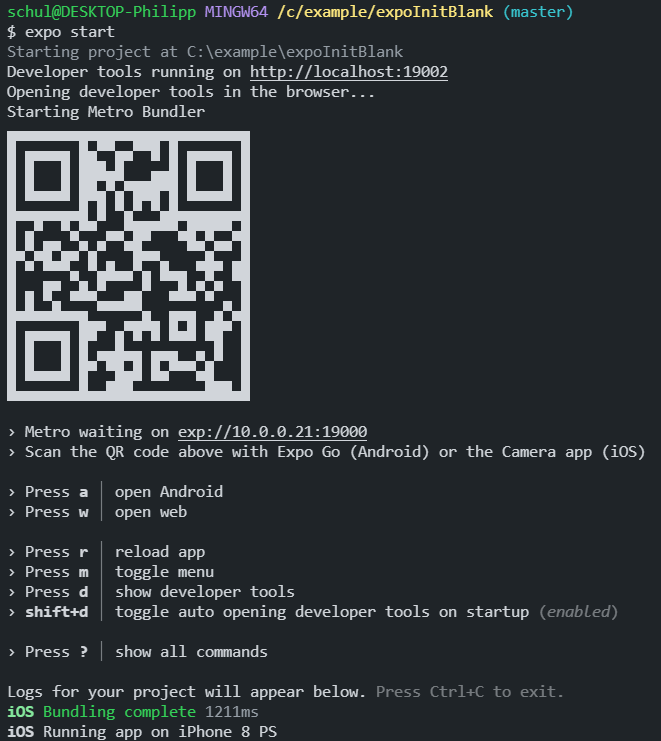
\includegraphics[width=0.6\textwidth]{Theorie/ReactNative/ExpoStart.png}
    \caption{Expo beim Start}
  \end{center}
\end{figure}

\begin{figure}[H]
  \begin{center}
    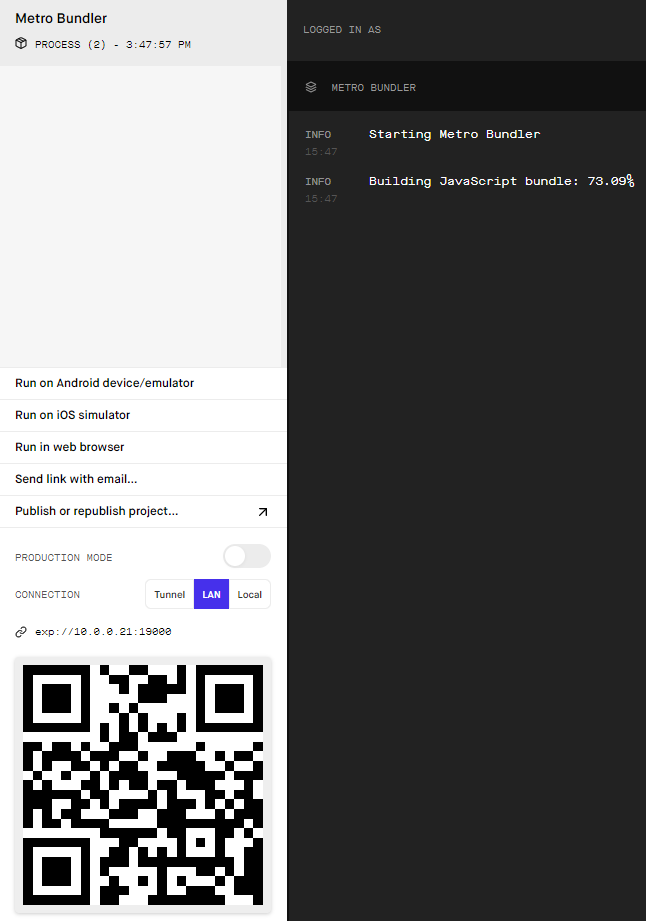
\includegraphics[width=0.6\textwidth]{Theorie/ReactNative/ExpoWebClient.png}
    \caption{Webinterface von Expo}
  \end{center}
\end{figure}

Nach dem Start wird im Webbrowser ein Entwickler-Menü geöffnet, auf dem noch einmal der QR-Code
und noch einige weitere hilfreiche Funktionen zu finden sind.

Um nun die App zu testen, muss man noch die ExpoGo App auf seinem Mobiltelefon installieren und den
gezeigten QR-Code scannen, während man im selben Netzwerk ist. Danach wird eine Bundle-Anfrage an
den lokalen Metro-Server geschickt, er kompiliert unser Projekt und schickt es an den Client.

\begin{figure}[H]
  \begin{center}
    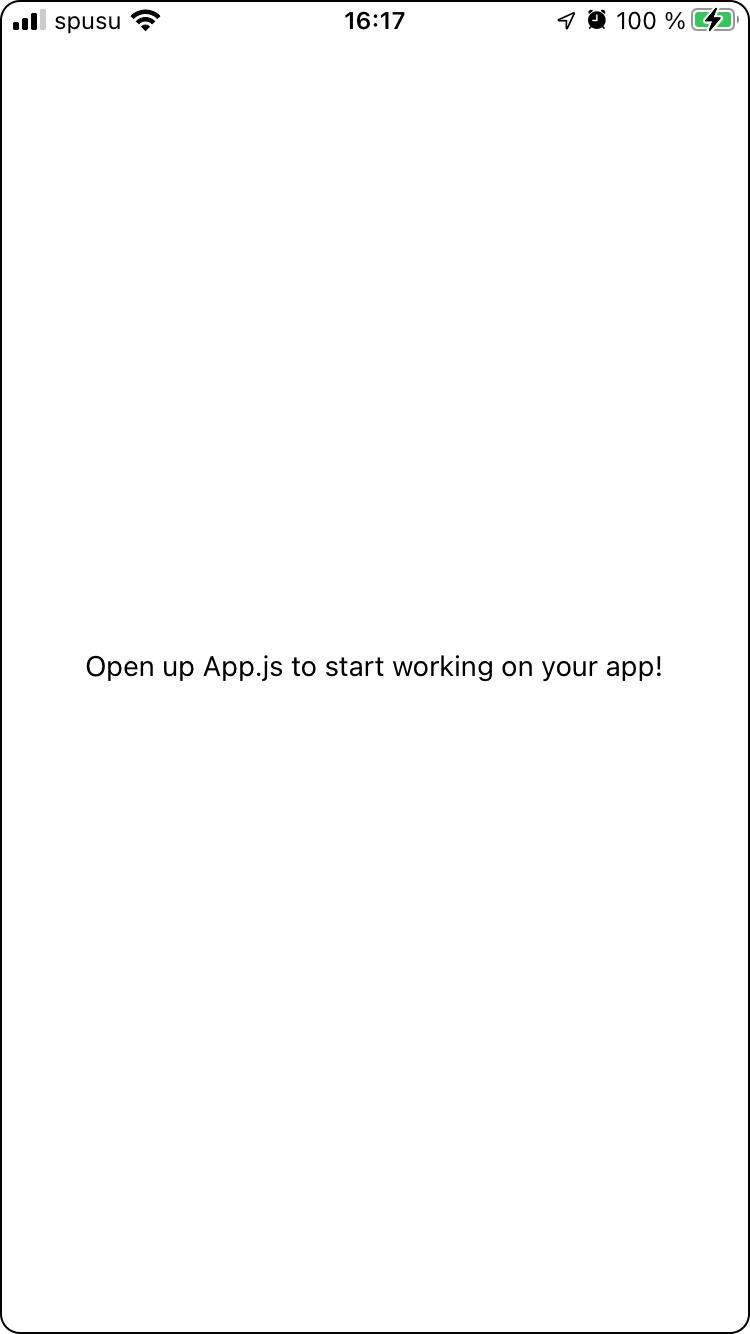
\includegraphics[width=0.5\textwidth]{Theorie/ReactNative/ExpoBlank.jpeg}
    \caption{Die weiße Leinwand von Expo}
  \end{center}
\end{figure}

\subsubsection{Expo Eject}
Wie bereits vorher schon erwähnt, hat es einige Nachteile seine App mit Expo zu machen. Um aber
einen schnellen Prototypen zu bauen ist das Framework perfekt. Um also eine Expo App in eine
vollwertige React Native Anwendung umzuwandeln, benötigt man folgenden Befehl.

\begin{lstlisting}
C:\example\expoInitBlank> expo eject
\end{lstlisting}

Man wird bei einer Eingabeaufforderung darüber informiert, dass dieser Prozess nicht rückgängig
gemacht werden kann. Danach sieht die Ordnerstruktur so aus:

\begin{figure}[H]
  \begin{center}
    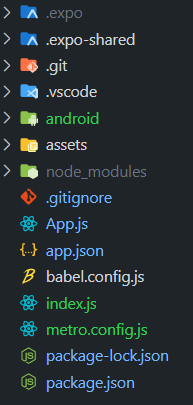
\includegraphics[height=0.5\textwidth]{Theorie/ReactNative/ExpoEject.png}
    \caption{Expo Eject Änderungen}
  \end{center}
\end{figure}

Um das Projekt für iOS-Geräte zu konfigurieren, führt man folgenden Befehl auf einem MacOS-PC aus:

\begin{lstlisting}
C:\example\expoInitBlank> npx pod-install
\end{lstlisting}

